\chapter{Full Visual Odometry}
% Title ideas: 
% Visual Odometry with Deep Learning
% Visual Odometry
% The Full Visual Odometry Pipeline

	\section{Introduction}
	% Describe the Task
	% Prior Work -> Flownet, DeepVO, VINet
	%
	The bulk of this chapter and the following experiments are based on the work of \cite{wang2017deepvo}.
	At the time of writing this thesis, \citeauthor{wang2017deepvo} have not released the source code of their implementation.
	Therefore, the aim of this chapter is to study and re-implement the ideas presented in their paper and to further expand on it.
	
	\section{Datasets}
		\todo{intro text}
		\begin{figure}
			\centering
			\begin{subfigure}[b]{0.8\linewidth}
				\centering
				\includegraphics[width=\linewidth]{Images/Data/kitti-example-image}
				\caption{
					KITTI
					\label{fig:kitti-example-image}
				}
			\end{subfigure}%
			\\
			\begin{subfigure}[b]{0.8\linewidth}
				\centering
				\includegraphics[width=\linewidth]{Images/Data/viper-example-image}
				\caption{
					VIPER
					\label{fig:viper-example-image}
				}
			\end{subfigure}%
			\caption[Example images from different datasets]
					{Example images from different datasets.
					 \todo{choose different image with scene dynamics, and show more images per dataset}
					 \label{fig:example-images-from-datasets}}
		\end{figure}
		\subsection{KITTI}
			KITTI from Karlsruhe Institute of Technology \cite{geiger2013vision} is a dataset that contains many video frames captured from the roof of a driving car.
			Each video frame is labeled with ground truth data such as camera pose and 3D points from a velodyne laser scanner.
			The camera pose was obtained by combining the data from GPS and an IMU (inertial measurement unit) that was mounted to the car.
			The dataset has around 23k stereo pairs of images with size $1226 \times 370$ pixels captured at a frame rate of [FPS]\todo{find frame rate}.
			For the experiments in this thesis, only the images from the left camera are used.
			The dataset is divided into 22 sequences, each captured at a different location in the metropolitan area of Karlsruhe, Germany.
			For the public, the ground truth is only available for the first 11 sequences.
			The rest of the data is intended to be used for submissions to the KITTI Vision Benchmark Suite\footnote{\url{http://www.cvlibs.net/datasets/kitti/eval_odometry.php}} 
			online.
			In the experiments here, only the sequences 0 to 10 are used and divided into training- and test sets.
		
		\subsection{VIPER}
			The VIPER dataset \cite{richter2017playing} contains a mix of car driving and walking sequences, but all data was generated synthetically from the video game Grand Theft Auto 5 released in April 2015.
			With around 254k frames it is significantly larger that the KITTI dataset.
			There is a variety of ground truth data available, including camera pose, semantic class labels and 3D object bounding boxes.
			The camera poses have been directly extracted from the game engine and are therefore fully accurate, while other data such as the semantic labels were generated in a post-processing step.
			VIPER is subdivided into training, test, and validation sets with 134k, 70k, and 50k frames respectively.
			The splits contain diverse scenes at day and night across different scene types such as urban, suburban under various weather conditions.
			
		\subsection{GTA V}
		% Self made dataset
		% mention that code for viper is not available
		% link to github repository
		% explain how it was caputured
		% What type of data does it contain
		%	- walking, running, driving, standing, 
		%	- weather, light, dynamic scene
		%	- 
		
		\subsection{Preprocessing}
			Each dataset contains long sequences/videos of thousands of frames over several minutes of recording.
			Due to the high memory footprint, it is unfeasible to load a complete sequence and feed it to the network.
			Therefore the sequences are cut into subsequences of smaller sizes. 
			For most experiments here, the sequence size is 100 frames or less.
			Instead of creating a segmentation of the dataset, this method of extracting subsequences also allows to define an overlap between sequences.
			This is especially useful when the dataset is small, such as KITTI.
			
			Since resolution and aspect ratio of the images are different between the datasets, they are first proportionally resized to a height of 320 pixels and then the center region of $448 \times 320$ pixels is extracted.
			Fixing the input size across multiple datasets makes it possible to train the same network architecture for different data and make a more accurate comparison.
			Due to the cropping, the left and right boundaries of the image are removed.
			An alternative is to resize the images directly without regard to the aspect ratio.
			This leads to a loss in horizontal resolution which could impact the networks performance for horizontal motions, e.g., a rotation of the camera around the vertical axis.
			The alternative resizing method was not studied in this thesis, but the impact is expected to be minor.
			
			The ground truth poses also require preprocessing. 
			Each raw sequence has a corresponding text file that contains the $3 \times 4$ pose matrices for every frame.
			These poses are all relative to the coordinate system of the first frame in the sequence.
			In other words, the coordinate system of the first frame is the world coordinate system of all other frames in the sequence.
			Because the raw sequences are divided into subsequences, the ground truth poses need to be converted to poses that are relative to the first frame within each subsequence.
			\todo{Refer to math equations in introduction}
			
			
	\section{Encoding the Pose}
	% Text from intro
	
	
	\section{The Model}
	% Figure with the entire pipeline
	% - Figure showing optical flow ??
	% Feature extraction
	%	- Optical flow
	%	- features relevant for motion
	%	- Flow alone is not enough
	% 	- Other high-level representation
	% Pose estimation
	%	- LSTM transforms feature to pose
	%	- Uses history from poses seen before to make current estimate more precise
	%	- 
	% Loss function and optimization
	% mse loss on euler + translation
	% experiments show that euler works best
	% 
		The main architecture is shown in figure~\ref{fig:main-architecture}.
		\begin{figure}[t]
			\centering
			\includegraphics[width=\linewidth]{Images/Model/DeepVO-arch}
			\caption[Main architecture for visual odometry]
					{Main architecture for visual odometry.
					 Green: Input of consecutive frames.
					 Yellow: Feature extraction.
					 Blue: Pose estimation with recurrent connections.
					 \todo{ref paper for figure, or redo figure}
					 \label{fig:main-architecture}}
		\end{figure}
		It consists of two main parts, the feature extraction and the recurrent part that estimates the pose at each time step.
		The network takes two consecutive images as input, that is the frames at time $t$ and $t - 1$.
		In order to estimate the camera motion, the network has to extract high-level features that are related to motion. 
		There are a number of features that are not helpful for estimating motion, e.g. \todo{list...}.
		
		\emph{Optical flow} is a feature related to motion. 
		It is defined as a vector-valued function $u(\vectr{x}) \in \R^2$ at each point $\vectr{x}$ in the image $I_{t}$ describing the translation of the point in the next frame such that
		\begin{equation}
			I_{t}(\vectr{x}) = I_{t + 1}(\vectr{x} + u(\vectr{x})).
		\end{equation}
		This property is called the \emph{brightness constancy constraint}.
		
		The idea is to estimate the motion of the camera from the 
		
		The feature extraction is done with a CNN that is based on FlowNetS by \cite{dosovitskiy2015flownet}.
		
		
		\subsection{Feature Extraction}
		% Describe flownet, what is optical flow
		% pretrained
		% on what was flownet trained?
			\begin{table}[tb]
				\small
				\begin{center}
					\begin{tabular}{|l|c|c|c|c|}
						\hline
						Layer 		& Kernel size 		& Stride 		& Padding 		& Channels 		\\ \hline
						conv1 		& $7 \times 7$		& 2 			& 3 			& 64 			\\ \hline
						conv2 		& $5 \times 5$		& 2 			& 2 			& 128 			\\ \hline
						conv3 		& $5 \times 5$		& 2 			& 2 			& 256			\\ \hline
						conv3.1 	& $3 \times 3$		& 1 			& 1 			& 256 			\\ \hline
						conv4 		& $3 \times 3$		& 2 			& 1 			& 512 			\\ \hline
						conv4.1 	& $3 \times 3$		& 1 			& 1 			& 512 			\\ \hline
						conv5 		& $3 \times 3$		& 2 			& 1 			& 512 			\\ \hline
						conv5.1 	& $3 \times 3$		& 1 			& 1 			& 512 			\\ \hline
						conv6 		& $3 \times 3$		& 2 			& 1 			& 1024 			\\ \hline
						conv6.1 	& $3 \times 3$		& 1 			& 1 			& 1024 			\\ \hline
					\end{tabular}
				\end{center}
				\caption[Architecture of the feature extraction based on FlownetS]
						{Architecture of the feature extraction based on FlownetS. 
						 Each layer is followed by a rectified linear unit (ReLU).}
				\label{tbl:first_part_of_flownets}
			\end{table}
		
		\subsection{The LSTM}
		% How does LSTM use flow features 
		% Table with fc layer and dropout
	
		\begin{table}[tb]
			\small
			\begin{center}
				\begin{tabular}{|l|c|c|}
					\hline
					Layer 		& Input size 					& Output size			\\ \hline
					lstm1 		& $1024 \cdot 5 \cdot 7$		& $1000$  				\\ \hline
					lstm2 		& $1000$						& $1000$ 				\\ \hline
					drop		& $1000$						& $1000$				\\ \hline
					fc 			& $1000$						& $6$					\\ \hline
				\end{tabular}
			\end{center}
			\caption[Architecture of the recurrent part of the pose network]
					{Architecture of the recurrent part of the pose network.
					 It consists of a two-layer LSTM with hidden size 1000, a dropout- and fully-connected layer.}
			\label{tbl:lstm_and_fc_after_flownet}
		\end{table}
	\section{Experiments and Results}
	% Ablation studies
	% Problem with "global" pose -> incremental pose
	% Training
	%	- Different learning rate for pretrained flownet
	%	- Dropout Regularization
	
		\begin{table}[tb]
			\small
			\begin{center}
				\begin{tabular}{|c|c|c||c|c|c|}
					\hline
					Length 	& Overlap 	& Dropout	& Total 	& Rotation	& Translation	\\ \hline
					25		& 0			& 0			& 19.0293	& 0.4981	& 18.5312		\\ \hline
					25		& 20		& 0			& 16.5471	& 0.3913	& 16.1558		\\ \hline
					100		& 20		& 0			& 529.9459	& 39.8967	& 490.0493		\\ \hline
					100 	& 5			& 0.5		& 376.7666	& 43.1578	& 333.6088		\\ \hline
					100		& 80		& 0			& 313.1278	& 47.8437	& 265.2841		\\ \hline
				\end{tabular}
			\end{center}
			\caption[Experiments on KITTI: Overlap and dropout]
					{Experiments on KITTI: Overlap and dropout. 
					 Shown is the test error on sequence 10 for different overlap and dropout during training.
					 Each model was trained with default parameters for 100 epochs.
					 \todo{also include growing sequence?}
					 \label{tbl:kitti-overlap-and-dropout}}
		\end{table}
		
		\begin{table}[tb]
			\small
			\begin{center}
				\begin{tabular}{|c|c||c|c|c|}
					\hline
					Training length & Test length 	& Total 	& Rotation	& Translation	\\ \hline
					25				& 25			& 16.5471	& 0.3913	& 16.1558		\\ \hline
					25				& 100			& 1060.7528	& 37.6196	& 1023.1332		\\ \hline
					100				& 100			& 529.9459	& 39.8967	& 490.0493		\\ \hline
				\end{tabular}
			\end{center}
			\caption[Experiments on KITTI: Testing on longer sequences]
					{Experiments on KITTI: Testing on longer sequences. 
					 When testing on longer sequences, the error becomes extremely high compared to the model trained on 100 frames.
					 \label{tbl:kitti-testing-on-longer-sequences}}
		\end{table}
	
		\begin{figure}
			\centering
			\begin{subfigure}[b]{0.5\linewidth}
				\centering
				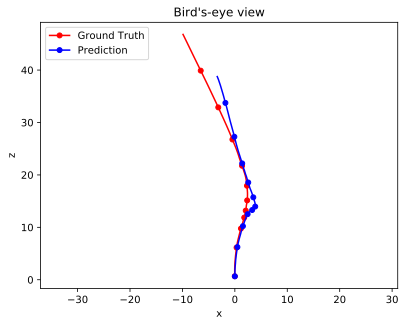
\includegraphics[width=\linewidth]{Images/Experiments/trained-on-25-frames}
				\caption{
					\label{fig:0}
				}
			\end{subfigure}%
			\begin{subfigure}[b]{0.5\linewidth}
				\centering
				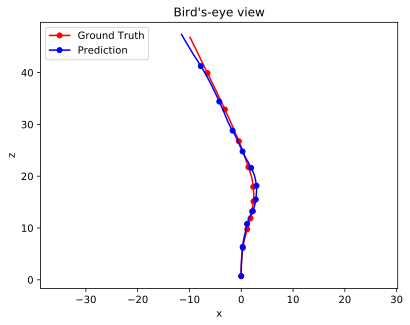
\includegraphics[width=\linewidth]{Images/Experiments/trained-on-100-frames}
				\caption{
					\label{fig:1}
				}
			\end{subfigure}%
			\caption[Training and testing on different sequence length]
					{Training and testing on different sequence length. 
					 Two models tested on a KITTI subsequence of 100 frames and trained on sequences of (a) 25 frames and (b) 100 frames. 
					 The markers in the plot are shown every ten frames.
					 \label{fig:kitti-testing-on-longer-sequences}}
		\end{figure}
	
		\begin{figure}
			\centering
			\begin{subfigure}[b]{\linewidth}
				\centering
				\includegraphics[width=0.45\linewidth]{example-image-a}
				\includegraphics[width=0.45\linewidth]{example-image-a}
				\caption{
					Long, curve
					\label{fig:0}
				}
			\end{subfigure}%
			\\
			\begin{subfigure}[b]{\linewidth}
				\centering
				\includegraphics[width=0.45\linewidth]{example-image-b}
				\includegraphics[width=0.45\linewidth]{example-image-b}
				\caption{
					Short
					\label{fig:0}
				}
			\end{subfigure}%
			\\
			\begin{subfigure}[b]{\linewidth}
				\centering
				\includegraphics[width=0.45\linewidth]{example-image-c}
				\includegraphics[width=0.45\linewidth]{example-image-c}
				\caption{
					\label{fig:0}
				}
			\end{subfigure}%
			\caption[Qualitative results for motion estimation on KITTI]
					{Qualitative results for motion estimation on KITTI.
					 Left column: Visualization of the estimated and true path.
					 Right column: Plot of each coordinate axis.
					 Markers are shown for every \todo{xx} frames.
					\label{fig:0}}
		\end{figure}
	
	
		\begin{figure}
			\centering
			\begin{subfigure}[b]{\linewidth}
				\centering
				\includegraphics[width=0.45\linewidth]{example-image-a}
				\includegraphics[width=0.45\linewidth]{example-image-a}
				\caption{
					Long, curve
					\label{fig:0}
				}
			\end{subfigure}%
			\\
			\begin{subfigure}[b]{\linewidth}
				\centering
				\includegraphics[width=0.45\linewidth]{example-image-b}
				\includegraphics[width=0.45\linewidth]{example-image-b}
				\caption{
					Short
					\label{fig:0}
				}
			\end{subfigure}%
			\\
			\begin{subfigure}[b]{\linewidth}
				\centering
				\includegraphics[width=0.45\linewidth]{example-image-c}
				\includegraphics[width=0.45\linewidth]{example-image-c}
				\caption{
					\label{fig:0}
				}
			\end{subfigure}%
			\caption[Qualitative results for motion estimation on VIPER]
					{Qualitative results for motion estimation on VIPER.
					 \label{fig:0}}
		\end{figure}
		
	\section{Discussion}
	\section{Conclusion}
